\chapter{Collective Problem Solving Patterns}\label{CPSP}

We have seen in the previous chapter how the ADELFE methodology was used for the design of AMAS, from the general requirement to the implementation of the agents. However a current limitation of ADELFE (shared with most of the existing comparable methods) comes from the fact that it is a general method, which aims to be applicable for design MAS intended for diverse application fields (problem solving, simulation, \emph{etc.}). This desire to be usable in a large spectrum of applications has the drawback that the recommendations and guidelines of ADELFE are of an bastract nature. This make the task of actually designing an AMAS for a precise application difficult for non agent expert, even when the application domain is narrower than, for example, general continuous optimization.\\
This limitation has already been observed in previous works, and has given birth to an ongoing effort to provide a modular toolkit named \emph{AMAS for Optimization (AMAS4Opt)}, with the goal to supplement ADELFE and assist AMAS designers when designing MAS for problem solving. In the same way that some contributions have already been proposed in the context of continuous optimization (see \cite{Ka2011.6}), we will now see how we can propose to enrich the toolkit in the context of continous optimization.

In this chapter, we take a step back from the MAS we described in the preceding parts and see how our contribution can be made more general, not only to the benefit of the scientific community, but also for engineers by enriching the AMAS4Opt. Numerical optimization was a mostly unexplored application domain in regard to multi-agents based algorithms. By taking the (somewhat ambitious) task to propose a MAS which would be applicable for this domain in its entirety, some of the patterns identified and some of the mechanisms we proposed can be used in a more general context than our system.

As numerical optimization is in itself an abstract mathematical field, we too had to abstract ourselves from concrete applications. We did not have the possibility to reduce the set of possible configurations and thus we had the occasion to encounter a variety of problems which have been mostly ignored before. Indeed, the graph representations of numerical optimization problems are quite diverse, and can present some topological properties not present in existing MAS formalisms. [[DCOP for example (presented in [[REF]]), ]]

In the description of our system, we presented a set of NCS [[use acronym ?]], and the specifics mechanisms we introduced to handle them. We believe that these NCS are only the instantiation of more general problematic configuration, which we dub \emph{Collective Problem Solving Patterns} (CPSP). The patterns are not restricted to numerical optimization, they can potentially be encountered in all sorts of application domains.

Architecture and software development has greatly benefited from the identification of common design pattern. In the same regard, we believe that the identification of these problem patterns as such, as well as of solution proposals to handle them, could lead to a great improvement for the design of agent-based systems for problem solving as a whole.

Consequently, we will present in this part how the NCS we identified during the design of our system can be abstracted in the broader form of CPSP.


\section{Introduction - Collective Problem Solving Patterns are not Design Patterns}

[[EXPLAIN THE DIFFERENCE WITH EXISTING AGENT PATTERNS]]

Before describing the CPSP in themselves, we must explain how these patterns differ from the existing design patterns for MAS.

There is already an existing (if limited) corpus of design patterns for MAS. These patterns have usually in scope either the design of the organizational structure of system or the design of the behavior architecture of the agents. These patterns concerns the \emph{design} of the system regarding the target application domain. These patterns are relevant in the design of the \emph{organization of the system}, according to the application domain.
What we propose here is a different sort of patterns, which concerns the \emph{behavior of the agent}, according to an existing organization. Design Patterns concern the structural aspects of the system, while Problem Solving Patterns concerns its functional aspects.

In this regard, CPSP are less generic than Design Patterns. Indeed the latter can be applied to the whole range of MAS, while the former only concerns MAS designed for problem solving (excluding, for example, MAS for simulation).

These two kinds of patterns should be seen as complementary. First the designer could use design pattern to design the structure of the MAS according to the needs of the application domain. Then he could use CPSP to identify and solve specific problems resulting from such modeling.

As we want a description of our patterns which is domain-free, we cannot re-use the modeling we introduced in \ref{modeling}. The NDMO formalism is indeed bound to the domain of numerical optimization. Consequently, we will now introduce a higher-level formalism, which concentrates on the relations between the agents of the system. to keep this formalism short and simple, we will make some assumptions about the functioning of the system.

We will consider systems composed of autonomous agents and resources. An agent may needs for one or more resources to be in a specific state to accomplish its local goal. We will suppose that a resource is controlled by one agent and one agent only. We believe that this simplifying assumption does not impede on the generality of the formalism (for example a system where two agents share the control of a resource can be viewed as equivalent to a system where both agents send requests to a third one solely in charge of it).

[[are these assumptions correct ??]]
To formalize the resources, we will consider each resource as a variable which can be assigned a number from a set representing its different possibles states. As most multi-agent systems manipulate numeric values, or data which can be represented by numeric values, this representation can be translated quite straightforwardly to most specifics cases.
The states represented by these numbers can be inherent to the resource, such as a color assigned to it in the graph coloring problem, or indicate the fact that the usage of the resource is attributed to a specific agent as in auction-based systems.

We will suppose that agents interact among themselves by message passing.

\section{Description of a Problem Solving Pattern}

\subsection{Agent Roles}\label{CPSP_roles}

Concerning the patterns we present in this article, we identified three different types of agent \emph{roles}: Provider, Solicitor and Transformer.

The \emph{Provider} role represents the fact that the agent is in charge of a given resource, which can be of use to others agents in the system. The agent is responsible of choosing the state of the resource or giving access to it based on solicitations of others.

The \emph{Solicitor} role represents the fact that the agent requires some resource(s) which it does not control to be in a specific state, in order to accomplish its goal. Consequently, the agent needs to solicit the agent(s) controlling the relevant resource(s).

The \emph{Transformer} role is a combination of the Provider and Solicitor roles. The transformer agent controls a resource but the state of the resource is dependent of some other resources not controlled by the agent. While this role can be represented by assigning both Provider and Solicitor roles to the agent, we found it common enough to be worth of a specific representation. As we will see, transformer agents sometimes play a specific role in the CPSP, as they can be a source of delay or obfuscation of information.

On \figurename{} \ref{cpsp_class_diag} is shown the very simple class diagram representing the relationships between these three roles.

\begin{figure}
\centering
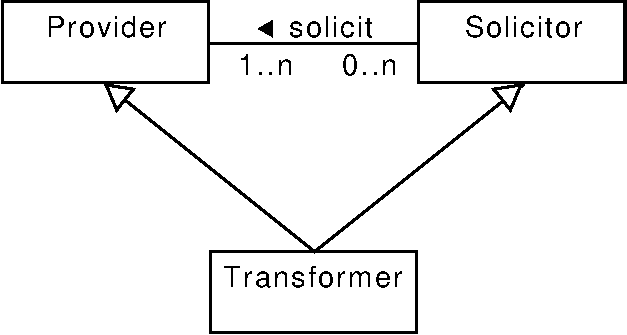
\includegraphics[width=0.5\textwidth]{cpsp_class_diag-crop}
\caption{class diagram of the Provider-Solicitor modeling.}
\label{cpsp_class_diag}
\end{figure}

It is important to understand that an agent is not limited to one role only. For a given system an agent can, depending on the context, assume any combination of these roles. Thus an agent can both solicit others agents regarding a resource, while providing a controlled resource to others agents.
In this regard, an agent can even be a producer and solicitor of the same resource. For example the agent is in charge of a specific resource, but also benefit from it. In this case the agent can possibly be in conflict with others agents regarding the state of the resource, and decide (as a producer) to go against its own interest (as a solicitor) in order to help another agent deemed more important.
Obviously, in most implementations, the different roles of the agent would not be as much segregated, and the agent would not strictly communicate with itself using message-passing. This distinction should not be a problem in practice (this kind of configuration can however trigger others CPSP, see for example \ref{NCS_async}).

For example, in the case of our system the different agent types had relatively defined and fixed roles. A design variable agent linked with at least one other agent has a \emph{provider} role. Constraint and objectives agents are \emph{solicitors}. Models agents have a \emph{transformer} role, as for output agents which are in input of at least one model or criterion agents.\\
The only agents which do not have a role corresponding to this taxonomy are the variable and output agents which are not used as input by any other agent. And indeed in our system these agents would have a basically non-existent role. Of course the user can still manually intervene to change the topology of the problem, changing at the same time the roles of these agents.

\subsection{Pattern Description}

For each CPSP, we provides a short description. This description will obviously be quite similar to the description of the NCS[[s]] in \ref{NCS_pres}, as they correspond to the same pattern, only from different abstraction levels.

As we already presented the details of the different mechanisms in section \ref{NCS_pres}, we will not detail them again in this part. Moreover, the CPSP aim to be general patterns applicable to multiple domains, consequently it is not possible to fully specify them. A part of the instantiation work still must be done by the designer. However we discuss some conditions which are necessary in order to instantiate the resolution mechanisms we proposed to the domain.

For each CPSP, we also provide a synthetic \enquote{blueprint} which is composed of two parts:
\begin{compactenum}
\item a representative agent configuration of the CPSP (using the agent roles introduced in section \ref{CPSP_roles}) 
\item a summary of the mechanisms involved in the solving of the CPSP.
\end{compactenum}
These blueprints are based on the template shown on \figurename{} \ref{blueprint_template}.

\begin{figure}
\centering
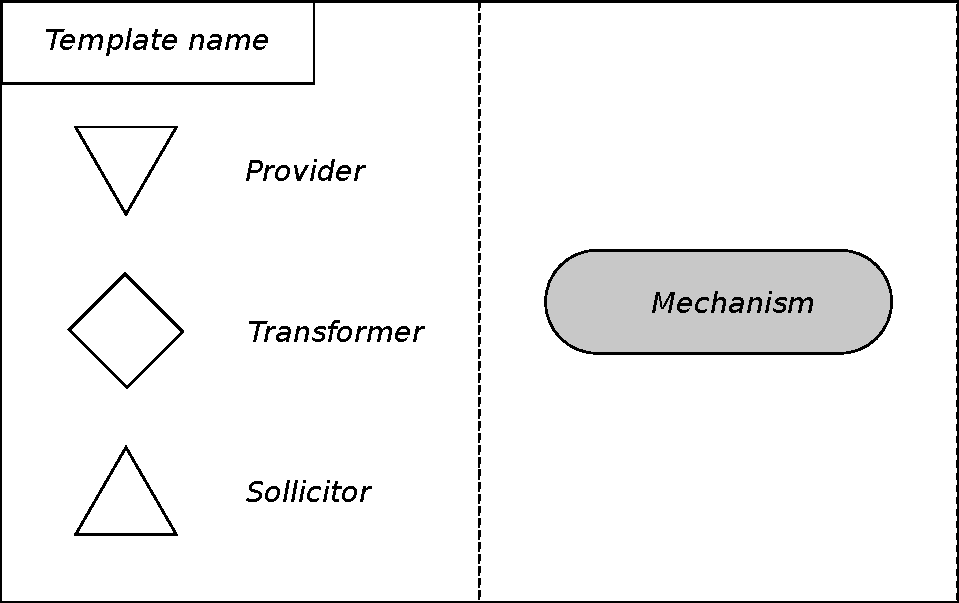
\includegraphics[width=0.6\textwidth]{blueprint_template}
\caption{Template on CPSP blueprints.}\label{blueprint_template}
\end{figure}

\section{Identified Collective Problem Solving Patterns}

In this section, we present the CPSP we identified from the NCS we encountered during the design of our MAS.

\subsection{Conflicting Requests}

In this situation a provider agent is requested to do different conflicting actions from several solicitors agents. This CPSP is probably the simplest one and was already identified as a recurring situation in previous works, since it is the direct instantiation of a NCS category (as presented in section \ref{amas_theory}).

The blueprint of this CPSP is shown on \figurename{} \ref{blueprint_conflicts}.

\begin{figure}
\centering
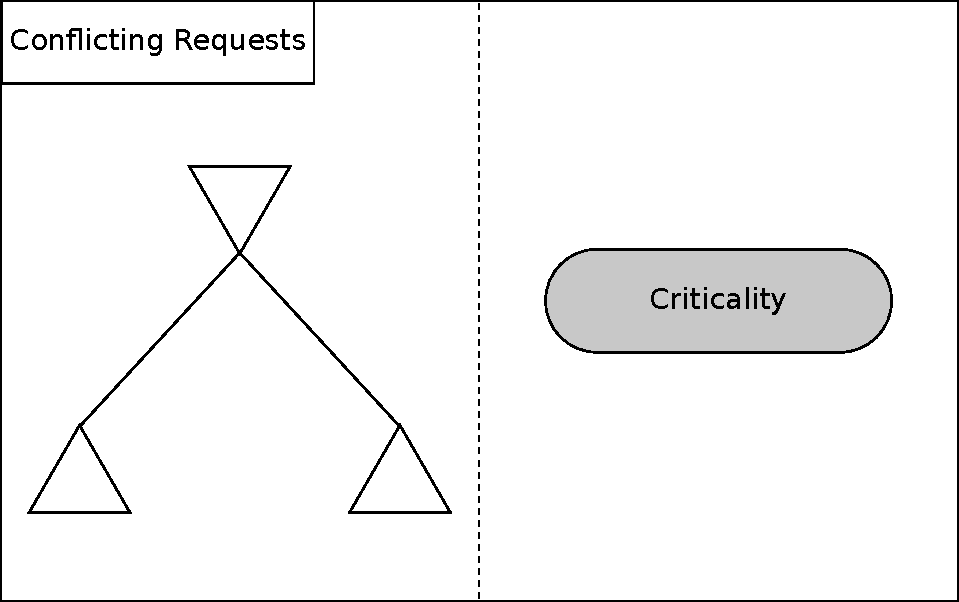
\includegraphics[width=0.6\textwidth]{blueprint_conflicts}
\caption{Conflicting Requests blueprint.}\label{blueprint_conflicts}
\end{figure}

In order to apply the blueprint, the designer must be able to define a common and comparable measure of the \enquote{dissatisfaction} state of the solicitors. This \emph{criticality} must be transmitted with the requests made by the solicitor agent.


The use of a criticality measure as way to discriminate between the different requests is a \enquote{tried-and-true} technique which has been applied to multiple AMAS applications [[cite some]].\\
As a remark, a measure of dissatisfaction present an advantage over a measure of satisfaction in the fact that it is often possible to estimate the state of maximal satisfaction of the agent (every requirement is perfectly satisfied), but not always possible to do so for the maximal dissatisfaction. Consequently a measure of satisfaction would have a upper bound but no lower bound, while a measure of dissatisfaction has a lower bound and no upper bound. This latter is easier to manipulate and reason with as it can be easily be represented by an unbounded positive value.

\subsection{Cooperative Trajectories}

[[TODO]]

\begin{figure}
\centering
	\begin{subfigure}{0.49\textwidth}
		\centering
		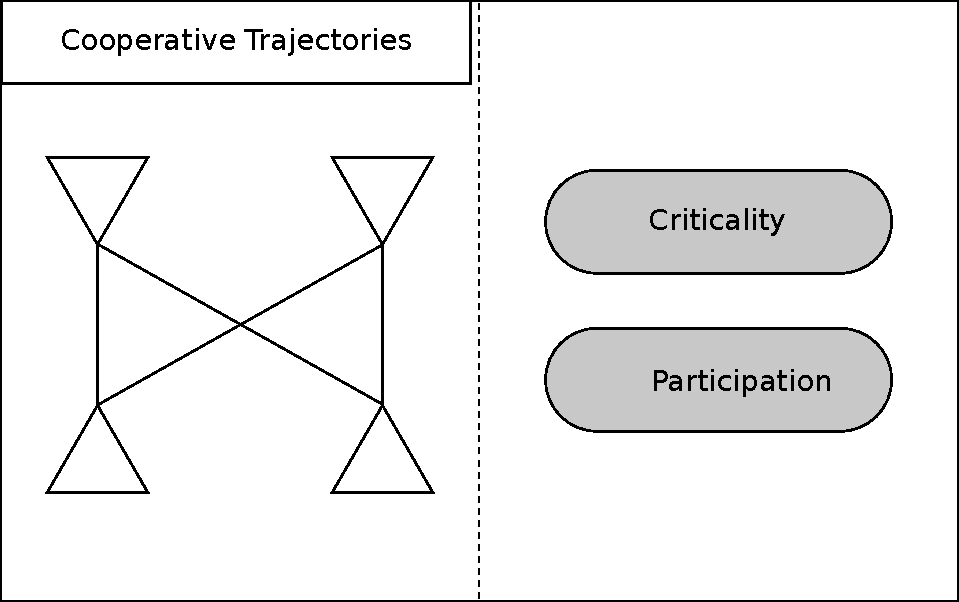
\includegraphics[width=\textwidth]{blueprint_coop_traj_var.pdf}
		\caption{Direct.}
	\end{subfigure}
	\begin{subfigure}{0.49\textwidth}
		\centering
		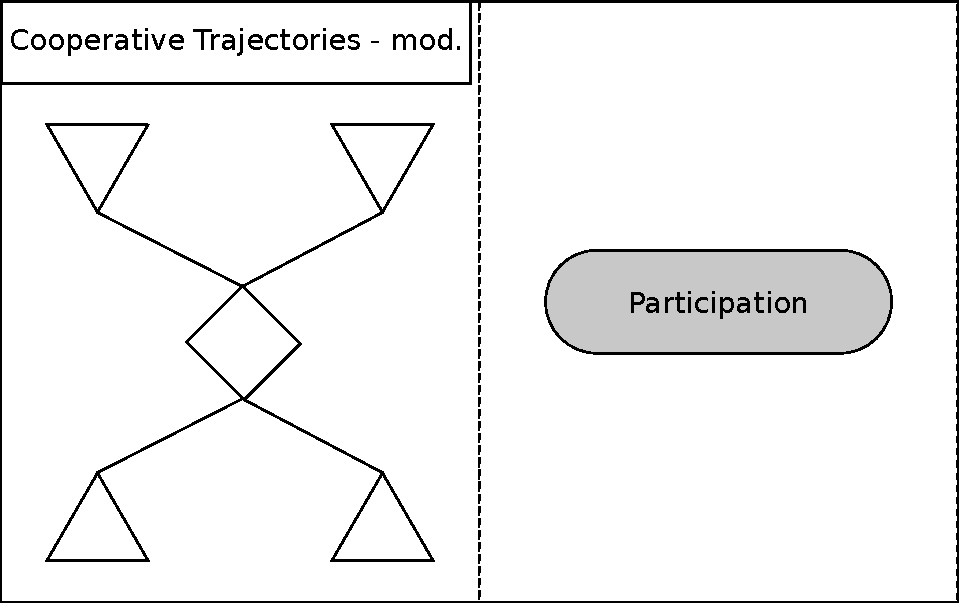
\includegraphics[width=\textwidth]{blueprint_coop_traj_model.pdf}
		\caption{With a Transformer agent.}
	\end{subfigure}
\caption{Cooperative Trajectories.}\label{blueprint_coop_traj}
\end{figure}

[[REALLY DO TWO FIGURES ? ONE IS BASICALLY A VARIANT OF THE OTHER]]

\subsection{Cycle Solving}

[[TODO]]

\begin{figure}
\centering
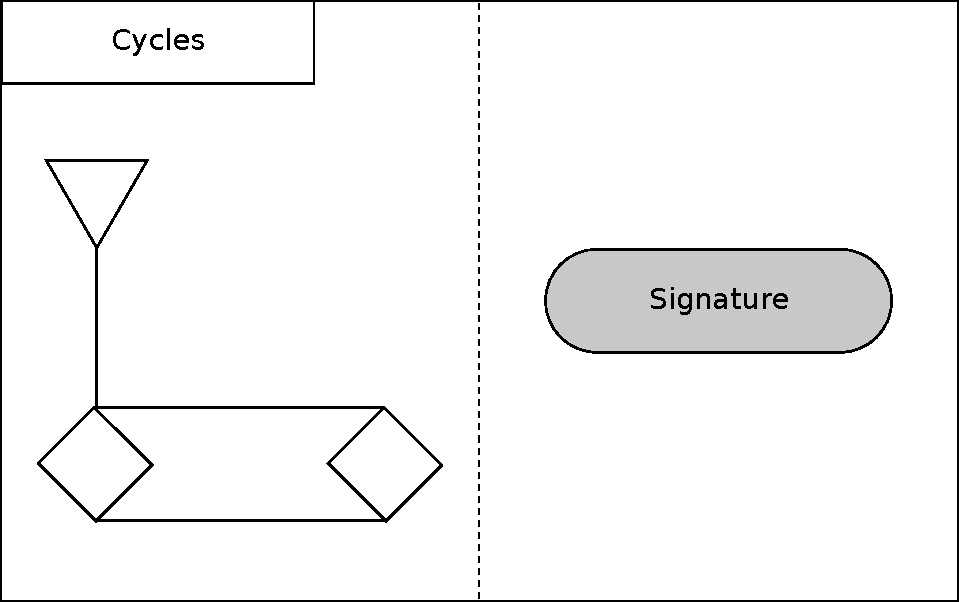
\includegraphics[width=0.6\textwidth]{blueprint_cycles}
\caption{Cycle Solving blueprint.}\label{blueprint_cycles}
\end{figure}

\subsection{Hidden Dependencies}

The hidden Dependency CPSP arises when a solicitor agent assumes the agents to which it sends requests are independent providers, while one of them is in fact dependent of the other (transformer role). This pattern leads to a suboptimal behavior when the solicitor agent sends requests which are contradictory to the \enquote{top-most} provider agent. The blueprint of this CPSP is shown on \figurename{} \ref{blueprint_hidden_dep}.

\begin{figure}
\centering
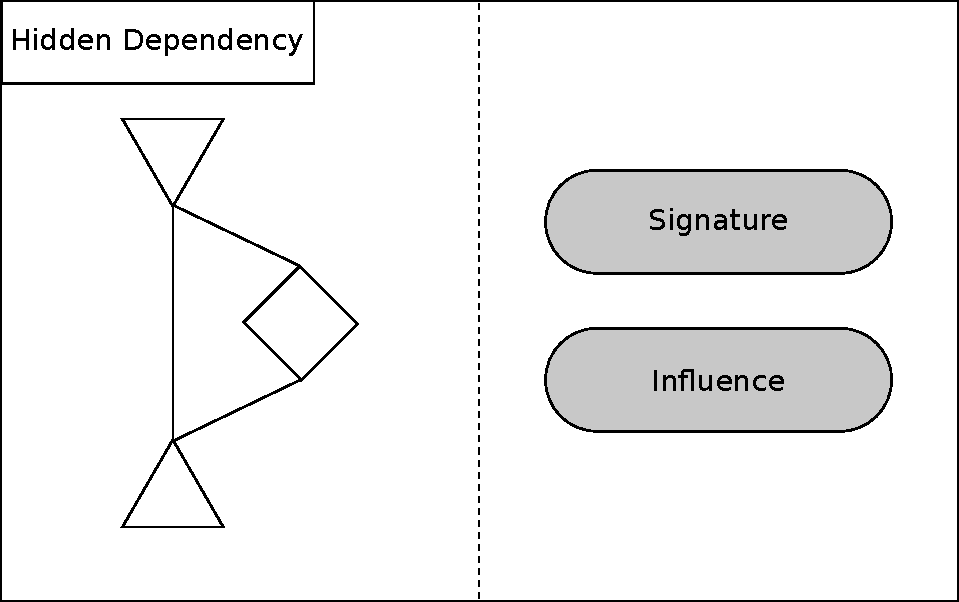
\includegraphics[width=0.6\textwidth]{blueprint_hidden_dep}
\caption{Hidden Dependencies blueprint.}\label{blueprint_hidden_dep}
\end{figure}

To apply this blueprint, the designer has to complement the messages exchanged by the agents with unique signatures containing an immutable \emph{origin} which uniquely identify the agent which is the origin of the request. The designer must also be able to define an \emph{influence} measure to be transmitted with the request, which represent the impact of the recipient on the solicitor. These \emph{influences} measures must be comparable for a same origin.

\subsection{Asynchronous Requests}

This CPSP arises when a provider agent receives requests from multiple solicitor agents, but these requests arrive in desynchronized manner. A possible suboptimal behavior can happen when the provider agent decides to satisfy a request from a solicitor, and receives afterward a more important request contradicting the first one. he blueprint of this CPSP is shown on \figurename{} \ref{blueprint_async}.

\begin{figure}
\centering
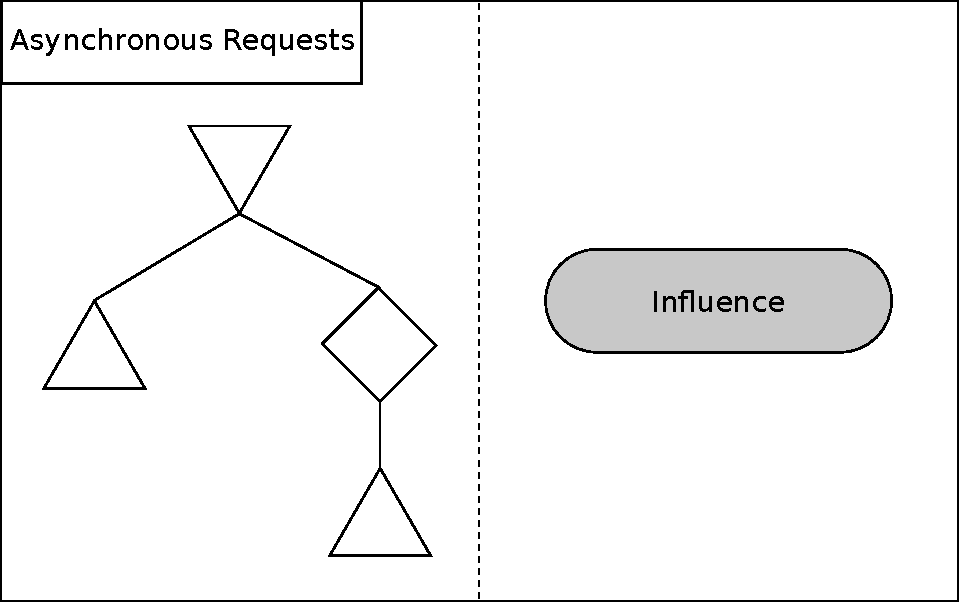
\includegraphics[width=0.6\textwidth]{blueprint_async}
\caption{Asynchronous Requests blueprint.}\label{blueprint_async}
\end{figure}

To apply this blueprint, the designer must be able to define an \emph{influence} measure for each solicitor agent to estimate, which represent the impact of the recipient on the solicitor. This \emph{influence} will allows the solicitor agent to determine when it received enough informations to make a sufficiently informed decision, without needing to wait for \emph{all} the answers to its requests.\\
Alternatively, if answer delay of the solicited agents is negligible, or if for any other reason it is deemed acceptable that a solicitor agent waits for all the answers before taking a decision, the mechanism can be adapted to avoid using \emph{influence} altogether.

\section{Conclusion on Collective Problem Solving Patterns}

[[TODO: add some text]]

We identified these patterns from the the NCS of our system. In reverse, the NCS used in the design of AMAS seems perfectly adequate to instantiate known CPSP. Indeed, subsumption-based behavior architectures are very appropriate to model this kind of \enquote{exception}-like situations. Should this kind of patterns identification and reuse becomes more wildly used, one could expect this way of modeling agent behavior to becomes quite popular.